% Options for packages loaded elsewhere
\PassOptionsToPackage{unicode}{hyperref}
\PassOptionsToPackage{hyphens}{url}
%
\documentclass[
]{book}
\usepackage{amsmath,amssymb}
\usepackage{lmodern}
\usepackage{ifxetex,ifluatex}
\ifnum 0\ifxetex 1\fi\ifluatex 1\fi=0 % if pdftex
  \usepackage[T1]{fontenc}
  \usepackage[utf8]{inputenc}
  \usepackage{textcomp} % provide euro and other symbols
\else % if luatex or xetex
  \usepackage{unicode-math}
  \defaultfontfeatures{Scale=MatchLowercase}
  \defaultfontfeatures[\rmfamily]{Ligatures=TeX,Scale=1}
\fi
% Use upquote if available, for straight quotes in verbatim environments
\IfFileExists{upquote.sty}{\usepackage{upquote}}{}
\IfFileExists{microtype.sty}{% use microtype if available
  \usepackage[]{microtype}
  \UseMicrotypeSet[protrusion]{basicmath} % disable protrusion for tt fonts
}{}
\makeatletter
\@ifundefined{KOMAClassName}{% if non-KOMA class
  \IfFileExists{parskip.sty}{%
    \usepackage{parskip}
  }{% else
    \setlength{\parindent}{0pt}
    \setlength{\parskip}{6pt plus 2pt minus 1pt}}
}{% if KOMA class
  \KOMAoptions{parskip=half}}
\makeatother
\usepackage{xcolor}
\IfFileExists{xurl.sty}{\usepackage{xurl}}{} % add URL line breaks if available
\IfFileExists{bookmark.sty}{\usepackage{bookmark}}{\usepackage{hyperref}}
\hypersetup{
  pdftitle={Desvendando Sistemas de Informação Geográfica},
  pdfauthor={Édipo Henrique Cremon},
  hidelinks,
  pdfcreator={LaTeX via pandoc}}
\urlstyle{same} % disable monospaced font for URLs
\usepackage{color}
\usepackage{fancyvrb}
\newcommand{\VerbBar}{|}
\newcommand{\VERB}{\Verb[commandchars=\\\{\}]}
\DefineVerbatimEnvironment{Highlighting}{Verbatim}{commandchars=\\\{\}}
% Add ',fontsize=\small' for more characters per line
\usepackage{framed}
\definecolor{shadecolor}{RGB}{248,248,248}
\newenvironment{Shaded}{\begin{snugshade}}{\end{snugshade}}
\newcommand{\AlertTok}[1]{\textcolor[rgb]{0.94,0.16,0.16}{#1}}
\newcommand{\AnnotationTok}[1]{\textcolor[rgb]{0.56,0.35,0.01}{\textbf{\textit{#1}}}}
\newcommand{\AttributeTok}[1]{\textcolor[rgb]{0.77,0.63,0.00}{#1}}
\newcommand{\BaseNTok}[1]{\textcolor[rgb]{0.00,0.00,0.81}{#1}}
\newcommand{\BuiltInTok}[1]{#1}
\newcommand{\CharTok}[1]{\textcolor[rgb]{0.31,0.60,0.02}{#1}}
\newcommand{\CommentTok}[1]{\textcolor[rgb]{0.56,0.35,0.01}{\textit{#1}}}
\newcommand{\CommentVarTok}[1]{\textcolor[rgb]{0.56,0.35,0.01}{\textbf{\textit{#1}}}}
\newcommand{\ConstantTok}[1]{\textcolor[rgb]{0.00,0.00,0.00}{#1}}
\newcommand{\ControlFlowTok}[1]{\textcolor[rgb]{0.13,0.29,0.53}{\textbf{#1}}}
\newcommand{\DataTypeTok}[1]{\textcolor[rgb]{0.13,0.29,0.53}{#1}}
\newcommand{\DecValTok}[1]{\textcolor[rgb]{0.00,0.00,0.81}{#1}}
\newcommand{\DocumentationTok}[1]{\textcolor[rgb]{0.56,0.35,0.01}{\textbf{\textit{#1}}}}
\newcommand{\ErrorTok}[1]{\textcolor[rgb]{0.64,0.00,0.00}{\textbf{#1}}}
\newcommand{\ExtensionTok}[1]{#1}
\newcommand{\FloatTok}[1]{\textcolor[rgb]{0.00,0.00,0.81}{#1}}
\newcommand{\FunctionTok}[1]{\textcolor[rgb]{0.00,0.00,0.00}{#1}}
\newcommand{\ImportTok}[1]{#1}
\newcommand{\InformationTok}[1]{\textcolor[rgb]{0.56,0.35,0.01}{\textbf{\textit{#1}}}}
\newcommand{\KeywordTok}[1]{\textcolor[rgb]{0.13,0.29,0.53}{\textbf{#1}}}
\newcommand{\NormalTok}[1]{#1}
\newcommand{\OperatorTok}[1]{\textcolor[rgb]{0.81,0.36,0.00}{\textbf{#1}}}
\newcommand{\OtherTok}[1]{\textcolor[rgb]{0.56,0.35,0.01}{#1}}
\newcommand{\PreprocessorTok}[1]{\textcolor[rgb]{0.56,0.35,0.01}{\textit{#1}}}
\newcommand{\RegionMarkerTok}[1]{#1}
\newcommand{\SpecialCharTok}[1]{\textcolor[rgb]{0.00,0.00,0.00}{#1}}
\newcommand{\SpecialStringTok}[1]{\textcolor[rgb]{0.31,0.60,0.02}{#1}}
\newcommand{\StringTok}[1]{\textcolor[rgb]{0.31,0.60,0.02}{#1}}
\newcommand{\VariableTok}[1]{\textcolor[rgb]{0.00,0.00,0.00}{#1}}
\newcommand{\VerbatimStringTok}[1]{\textcolor[rgb]{0.31,0.60,0.02}{#1}}
\newcommand{\WarningTok}[1]{\textcolor[rgb]{0.56,0.35,0.01}{\textbf{\textit{#1}}}}
\usepackage{longtable,booktabs,array}
\usepackage{calc} % for calculating minipage widths
% Correct order of tables after \paragraph or \subparagraph
\usepackage{etoolbox}
\makeatletter
\patchcmd\longtable{\par}{\if@noskipsec\mbox{}\fi\par}{}{}
\makeatother
% Allow footnotes in longtable head/foot
\IfFileExists{footnotehyper.sty}{\usepackage{footnotehyper}}{\usepackage{footnote}}
\makesavenoteenv{longtable}
\usepackage{graphicx}
\makeatletter
\def\maxwidth{\ifdim\Gin@nat@width>\linewidth\linewidth\else\Gin@nat@width\fi}
\def\maxheight{\ifdim\Gin@nat@height>\textheight\textheight\else\Gin@nat@height\fi}
\makeatother
% Scale images if necessary, so that they will not overflow the page
% margins by default, and it is still possible to overwrite the defaults
% using explicit options in \includegraphics[width, height, ...]{}
\setkeys{Gin}{width=\maxwidth,height=\maxheight,keepaspectratio}
% Set default figure placement to htbp
\makeatletter
\def\fps@figure{htbp}
\makeatother
\setlength{\emergencystretch}{3em} % prevent overfull lines
\providecommand{\tightlist}{%
  \setlength{\itemsep}{0pt}\setlength{\parskip}{0pt}}
\setcounter{secnumdepth}{5}
\usepackage{booktabs}
\ifluatex
  \usepackage{selnolig}  % disable illegal ligatures
\fi
\usepackage[]{natbib}
\bibliographystyle{apalike}

\title{Desvendando Sistemas de Informação Geográfica}
\author{Édipo Henrique Cremon}
\date{2021-06-07}

\begin{document}
\maketitle

{
\setcounter{tocdepth}{1}
\tableofcontents
}
\hypertarget{introduuxe7uxe3o-ao-sig}{%
\chapter{Introdução ao SIG}\label{introduuxe7uxe3o-ao-sig}}

É comum nos depararmos com uma série de nomenclaturas cuja diferenciação torna-se nebulosa até mesmo para quem está atuando na área há bastante tempo. É comum vermos pessoas usando os termos geoprocessamento, geotecnologias e SIG (Sistema de Informação Geográfica) como sinônimos. Mas não são! Inclusive há certa hierarquia dentro destes conceitos e iremos detalhar cada um a seguir.

\hypertarget{geoprocessamento}{%
\section{Geoprocessamento}\label{geoprocessamento}}

Corresponde ``a área do conhecimento que utiliza técnicas matemáticas e computacionais para o tratamento da informação geográfica e que vem influenciando de maneira crescente as áreas de Cartografia, Análise de Recursos Naturais, Transportes, Comunicações, Energia e Planejamento Urbano e Regional'' \citep{CamaraDavis2001}.

\hypertarget{geotecnologias}{%
\section{Geotecnologias}\label{geotecnologias}}

Podemos definir geotecnologias como:

\begin{itemize}
\item
  Conjunto de tecnologias para coleta, processamento, análise e disponibilização de informação com referência geográfica;
\item
  As geotecnologias são compostas por soluções em hardware, software e peopleware (recursos humanos) que juntos se constituem em poderosas ferramentas para tomada de decisão;
\item
  As geotecnologias estão entre os três mercados emergentes mais importantes da atualidade, junto com a nanotecnologia e a biotecnologia (Revista Nature, jan2004);
\end{itemize}

\hypertarget{sistemas-de-informauxe7uxe3o-geogruxe1fica---sig}{%
\section{Sistemas de Informação Geográfica - SIG}\label{sistemas-de-informauxe7uxe3o-geogruxe1fica---sig}}

As ferramentas computacionais para Geoprocessamento, chamadas de Sistemas de Informação Geográfica (SIG), permitem realizar análises complexas, ao integrar dados de diversas fontes e ao criar bancos de dados georreferenciados. Tornam ainda possível automatizar a produção de documentos cartográficos \citep{CamaraDavis2001}.

Podemos dizer que é convergência de diferentes disciplinas onde o espaço (computacionalmente representado) é a linguagem comum. Como inúmeros campos da ciência (geografia, geologia, agronomia, engenharias ambiental, florestal, cartográfica e agrimensura, do transporte, etc) tratam de dados com uma localização geográfica, logo o SIG se faz como uma poderosa ferramenta de análise destes campos.

Pode-se definir SIG como um conjunto de ferramentas computacionais composto de equipamentos e programas que por meio de técnicas, \textbf{integra dados} (das mais diversas fontes), pessoas e instituições, de forma a tornar possível a coleta, o \textbf{armazenamento}, a \textbf{análise} e a \textbf{disponibilização}, a partir de \textbf{dados georreferenciados}, de informações produzidas por meio de aplicações, visando maior facilidade, segurança e agilidade nas atividades humanas referentes ao monitoramento, planejamento e tomada de decisão relativas ao espaço geográfico.

\hypertarget{informauxe7uxe3o-geogruxe1fica-ig}{%
\section{Informação Geográfica (IG)}\label{informauxe7uxe3o-geogruxe1fica-ig}}

Por sua vez, a informação geográfica pode ser entendida como:

\begin{itemize}
\item
  Informação sobre lugares na superfície da Terra;
\item
  Conhecimento sobre onde alguma coisa está;
\item
  Conhecimento sobre o que está em uma dada localização (GOODCHILD, 1997).
\end{itemize}

Nesse contexto, o adjetivo ``geográfico'' corresponde a informação que está sobre a superfície da Terra. Dado essa restrição é comum ser usado o termo informação espacial, uma vez que o termo espacial não se restringe apenas a informações sobre a superfície terrestre, se referindo genericamente a qualquer lugar no espaço. Também é comum encontrar o termo informação geoespacial ou geoinformação que na prática, ao observarmos a etimologia da palavra, ``geo'' significa Terra, sendo assim informação geoespacial corresponde a toda informação no planeta Terra, não se restringindo a superfície, sendo um conceito mais abrangente que informação geográfica. Em ambiente SIG também é usual que diversas análises sejam denominadas de análise espacial, não análise geográfica, já que podem ser aplicadas a diversas finalidades que podem ser mais abrangentes que a algo que está sobre a superfície terrestre.

\textbf{Você sabe a diferença entre dado e informação? E conhecimento?}

No dia a dia ouvimos muitos termos relacionados como processamento de dados, sistemas de informação, gestão de conhecimento, arquitetura da informação, coleta de dados, base de conhecimentos, entre outros. Mas qual a diferença entre dados, informação e conhecimento?

Em linhas gerais, dados estão relacionados à números, textos, símbolos que são neutros que vistos isoladamente não possuem significado algum, ou seja, por si só não permitem transmitir qualquer mensagem para o entendimento de uma dada situação ou problema.

Quando os dados são tratados e passam a constituir algum significado, passamos a ter a informação. Logo, podemos dizer que a dados são códigos que constituem a matéria prima da informação.

Por sua vez, o conhecimento não seria o acesso a um grande volume de informação, segundo \citet{longley2013} o conhecimento pode ser considerado como a informação no qual foi agregado valor por uma interpretação com base num dado contexto particular, experiência e propósito.

\hypertarget{ciuxeancia-da-informauxe7uxe3o-geogruxe1fica}{%
\section{Ciência da Informação Geográfica}\label{ciuxeancia-da-informauxe7uxe3o-geogruxe1fica}}

Dado que a ciência da informação estuda os temas fundamentais decorrentes da criação, manuseio, armazenamento e uso da informação. Logo, a Ciência da Informação Geográfica estuda os temas decorrentes da IG.
Na bibliografia é comum constatar o uso dos termos ciência da informação geográfica, geomática, ciência da informação espacial e engenharia da geoinformação. De autor para autor esses termos podem ter ligeiras diferenças, mas em linhas gerais são denominações muito próximas.

\hypertarget{exemplo}{%
\chapter{Exemplo}\label{exemplo}}

This is a \emph{sample} book written in \textbf{Markdown}. You can use anything that Pandoc's Markdown supports, e.g., a math equation \(a^2 + b^2 = c^2\).

The \textbf{bookdown} package can be installed from CRAN or Github:

\begin{Shaded}
\begin{Highlighting}[]
\FunctionTok{install.packages}\NormalTok{(}\StringTok{"bookdown"}\NormalTok{)}
\CommentTok{\# or the development version}
\CommentTok{\# devtools::install\_github("rstudio/bookdown")}
\end{Highlighting}
\end{Shaded}

Remember each Rmd file contains one and only one chapter, and a chapter is defined by the first-level heading \texttt{\#}.

To compile this example to PDF, you need XeLaTeX. You are recommended to install TinyTeX (which includes XeLaTeX): \url{https://yihui.org/tinytex/}.

\hypertarget{visao}{%
\chapter{Visão Geral de um SIG}\label{visao}}

Há pelo menos três grandes maneiras de utilizar um SIG \citep{camaraqueiroz2001}:

\begin{itemize}
\item
  como ferramenta para produção de mapas;
\item
  como suporte para análise espacial de fenômenos;
\item
  como um banco de dados geográficos, com funções de armazenamento e recuperação de informação espacial.
\end{itemize}

A facilidade de trabalhar com a informação geográfica em ambiente SIG, seja na sua criação e/ou edição, tornou o trabalho dos cartógrafos mais facilitada, constituindo uma importante ferramenta tanta na cartografia sistemática, quanto na cartografia temática. Com as ferramentas robustas de visualização, simbologia e layout, mapas têm sido produzidos tanto para saídas gráficas em meio digital e para impressão, com destaque para a criação de webmaps, onde os mapas são acessados via web interativamente com o usuário.

O que torna o SIG um ambiente poderoso de trabalho em relação a pacotes dedicados a desenho (p.ex. CAD) é sua capacidade de análise espacial. Baseado em inúmeras ferramentas é possível cruzar, interpolar e agregar dados para se chegar novas informações, tendo a inferência geográfica como um grande campo a ser explorado. A disciplina de SIG-2 do nosso curso abordará em mais detalhe esse conteúdo.

Por fim, e não menos importante, deve-se destacar a capacidade de trabalhar com SIG como um ambiente gerenciamento de banco de dados geográficos. Em tempos, onde há um volume considerável de informações, trabalhar com banco de dados é imprescindível, se for dados geográficos, um banco de dados geográficos é ainda mais relevante. Os softwares de SIG permitem gerenciar esses bancos de dados com funções de armazenamento e recuperação da informação que facilitam e muito quando trabalhamos com grande quantidade de dados.

Nesse sentido, é possível indicar que as principais características de SIG são:

\begin{itemize}
\tightlist
\item
  Inserir e integrar, numa única base de dados, informações espaciais provenientes de dados cartográficos, dados censitários e cadastro urbano e rural, imagens de satélite, redes e modelos numéricos de terreno (informações geográficas);
\end{itemize}


\includegraphics[width=1.75in]{./images/sig_cad}

O SIG oferece mecanismos para combinar as várias informações, através de algoritmos de manipulação e análise, bem como para consultar, recuperar, visualizar e plotar o conteúdo da base de dados georreferenciados \citep{camaraqueiroz2001}.

\begin{itemize}
\item
  A diferença fundamental é na diversidade de dados utilizados para a realização de suas tarefas, sendo que um SIG utiliza muito mais dados do que um CAD;
\item
  O SIG realiza operações com dados vetoriais e matriciais (imagens ``raster''), enquanto os CADs se limitam a trabalhar com dados vetoriais;
\item
  SIG tem capacidade de tratar as relações espaciais entre os objetos geográficos. Denota-se por topologia a estrutura de relacionamentos espaciais (vizinhança, proximidade, pertinência);
\item
  O CAD é usado para desenhos de caráter técnico que variam desde projetos de aviões até projetos de circuitos integrados, podendo ser usado para geração de cartas;
\end{itemize}

• Geralmente nas aplicações de CAD, os desenhos não possuem atributos descritivos, mas apenas propriedades gráficas.

Fonte: \url{http://www.dpi.inpe.br/spring/portugues/tutorial/geracao.html}

\hypertarget{exemplo-1}{%
\chapter{Exemplo}\label{exemplo-1}}

You can label chapter and section titles using \texttt{\{\#label\}} after them, e.g., we can reference Chapter \ref{intro}. If you do not manually label them, there will be automatic labels anyway, e.g., Chapter \ref{methods}.

Figures and tables with captions will be placed in \texttt{figure} and \texttt{table} environments, respectively.

\begin{Shaded}
\begin{Highlighting}[]
\FunctionTok{par}\NormalTok{(}\AttributeTok{mar =} \FunctionTok{c}\NormalTok{(}\DecValTok{4}\NormalTok{, }\DecValTok{4}\NormalTok{, .}\DecValTok{1}\NormalTok{, .}\DecValTok{1}\NormalTok{))}
\FunctionTok{plot}\NormalTok{(pressure, }\AttributeTok{type =} \StringTok{\textquotesingle{}b\textquotesingle{}}\NormalTok{, }\AttributeTok{pch =} \DecValTok{19}\NormalTok{)}
\end{Highlighting}
\end{Shaded}

\begin{figure}

{\centering 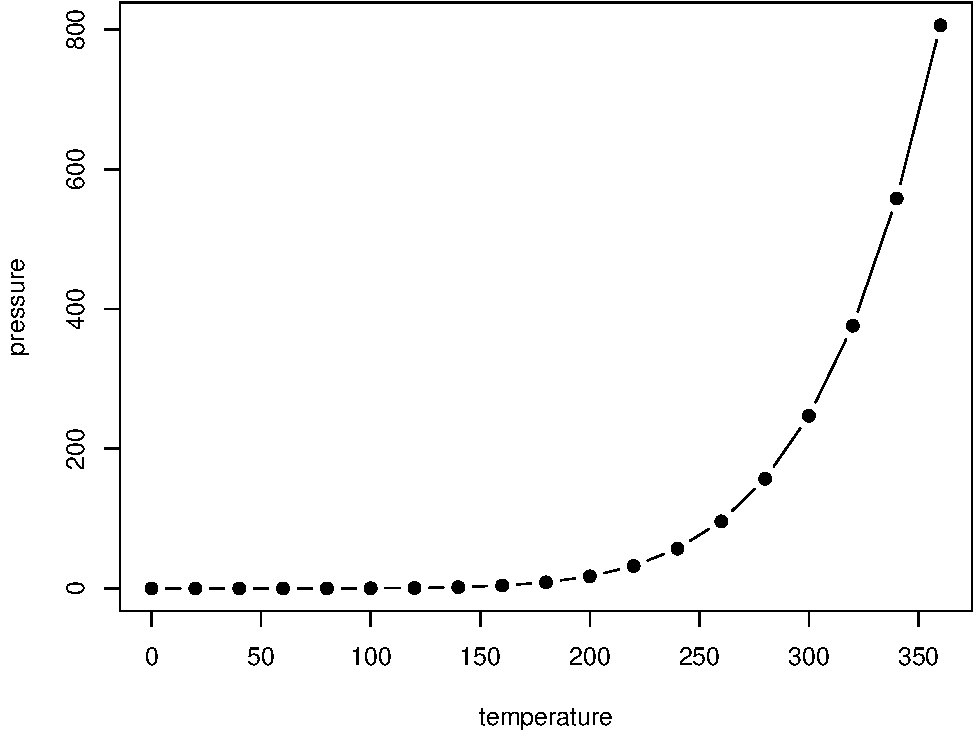
\includegraphics[width=0.8\linewidth]{livro_sig_files/figure-latex/nice-fig-1} 

}

\caption{Here is a nice figure!}\label{fig:nice-fig}
\end{figure}

Reference a figure by its code chunk label with the \texttt{fig:} prefix, e.g., see Figure \ref{fig:nice-fig}. Similarly, you can reference tables generated from \texttt{knitr::kable()}, e.g., see Table \ref{tab:nice-tab}.

\begin{Shaded}
\begin{Highlighting}[]
\NormalTok{knitr}\SpecialCharTok{::}\FunctionTok{kable}\NormalTok{(}
  \FunctionTok{head}\NormalTok{(iris, }\DecValTok{20}\NormalTok{), }\AttributeTok{caption =} \StringTok{\textquotesingle{}Here is a nice table!\textquotesingle{}}\NormalTok{,}
  \AttributeTok{booktabs =} \ConstantTok{TRUE}
\NormalTok{)}
\end{Highlighting}
\end{Shaded}

\begin{table}

\caption{\label{tab:nice-tab}Here is a nice table!}
\centering
\begin{tabular}[t]{rrrrl}
\toprule
Sepal.Length & Sepal.Width & Petal.Length & Petal.Width & Species\\
\midrule
5.1 & 3.5 & 1.4 & 0.2 & setosa\\
4.9 & 3.0 & 1.4 & 0.2 & setosa\\
4.7 & 3.2 & 1.3 & 0.2 & setosa\\
4.6 & 3.1 & 1.5 & 0.2 & setosa\\
5.0 & 3.6 & 1.4 & 0.2 & setosa\\
\addlinespace
5.4 & 3.9 & 1.7 & 0.4 & setosa\\
4.6 & 3.4 & 1.4 & 0.3 & setosa\\
5.0 & 3.4 & 1.5 & 0.2 & setosa\\
4.4 & 2.9 & 1.4 & 0.2 & setosa\\
4.9 & 3.1 & 1.5 & 0.1 & setosa\\
\addlinespace
5.4 & 3.7 & 1.5 & 0.2 & setosa\\
4.8 & 3.4 & 1.6 & 0.2 & setosa\\
4.8 & 3.0 & 1.4 & 0.1 & setosa\\
4.3 & 3.0 & 1.1 & 0.1 & setosa\\
5.8 & 4.0 & 1.2 & 0.2 & setosa\\
\addlinespace
5.7 & 4.4 & 1.5 & 0.4 & setosa\\
5.4 & 3.9 & 1.3 & 0.4 & setosa\\
5.1 & 3.5 & 1.4 & 0.3 & setosa\\
5.7 & 3.8 & 1.7 & 0.3 & setosa\\
5.1 & 3.8 & 1.5 & 0.3 & setosa\\
\bottomrule
\end{tabular}
\end{table}

You can write citations, too. For example, we are using the \textbf{bookdown} package \citep{R-bookdown} in this sample book, which was built on top of R Markdown and \textbf{knitr} \citep{xie2015}.

\hypertarget{literature}{%
\chapter{Literature}\label{literature}}

Here is a review of existing methods.

\hypertarget{methods}{%
\chapter{Methods}\label{methods}}

We describe our methods in this chapter.

\hypertarget{applications}{%
\chapter{Applications}\label{applications}}

Some \emph{significant} applications are demonstrated in this chapter.

\hypertarget{example-one}{%
\section{Example one}\label{example-one}}

\hypertarget{example-two}{%
\section{Example two}\label{example-two}}

\hypertarget{final-words}{%
\chapter{Final Words}\label{final-words}}

We have finished a nice book.

  \bibliography{book.bib,packages.bib}

\end{document}
